\subsection{Description of Data}
In order for the middleware and storage layer to understand data,
I/O intentions, and act accordingly, describing data in a way that can
be understood by the system is needed. In this project, this is achieved 
by managing data as \textit{objects}.
An object is the smallest unit of data that consists of raw data and metadata,
and a user space variable, such as \textit{temperature}, may consist of a collection
of objects possibly with different accuracy or resolution.
A key advantage of representing data as \textit{objects}, rather than 
bytes, is that it allows data semantics, user intentions, QoS requirements, and
the relationship between user data to be readily captured and embedded with the 
raw data. As an example, retrieving a 3D field data generated from a simulation 
and then visualizing it requires the coordinates and connectivity variable 
1) to be accessed together and 2) with low latency in order to achieve a good user experience. 
The description of data, as enabled by managing data as objects, bridges 
the semantics gap between applications, middleware, and storage systems,
and allows the system to understand user-level data, execute QoS requirements and policies, and
optimize application and system performance.

%The new APIs will enable the bridge by specifying selectable performance/quality/- cost tradeoffs 
%from both the application and system perspectives based upon the user guided rules/policy and 
%runtime system monitoring status. It allows the middleware to make best possible decisions from 
%the feedback of storage system knowledge, such that it will embed user intentions and the available 
%system storage. 
%We want the system to give the users a certain amount of currency 
%in terms of bandwidth, storage space on each level, and latency expectations. These notions will be fuzzy 
%but they will allow the user to make ad-hoc decisions to figure out what needs to be saved.

The description of data is essentially metadata and it may include conventional attributes, such as 
data type, size, dimensionality, relationship to other data, and etc. In particular,
relationship to other data objects can be captured by implementing \textit{soft links}
and different types of relationships can be expressed by different types of soft links. 
In this project, a key metadata attribute
that enables QoS scheduling, data placement, and lifetime, is \textit{data utility}, which
captures the priority of objects - it is to our belief that
for exascale science, users must prioritize a small set of objects to be saved on 
higher-level capacity-limited storage 
to avoid the slow access to large-capacity lower-level storage, such as tape.
We propose a new technique, described by a utility function plugged in by a user, 
where objects can be cast into multiple buckets of data, and each bucket can be prioritized 
differently according to its utility value.
Once this is done, the middleware system will construct the description of data, re-organize
and place data to achieve the desired QoS goals and policies.

In the meanwhile, the user would like the ability to get a certain amount of Quality of Service 
such that they can then make decisions when the expected bandwidth.
%for example is less than what they desire and will then place in a certain set 
%of rules which the system can make autonomic decisions to help decide what should be done.
A key insight in this proposed project has been the increased interaction of
the application with the storage system. Towards this end, we propose to
address the quality of service requirements by providing the application
with mechanisms to specify the quality of I/O service, interrogate the
storage system, and react to the responses. Guided by our past work in
ADIOS \cite{lofstead2008flexible} we propose to explore the design of two
mechanisms for this purpose. 

Our research will address the following questions: 1) How can users interact with the SSIO system efficiently?,
2) How can users express their intentions into actionable items which can take place in the SSIO layer?
3) How can users give utility to the data?


\paragraph{State of the art:} ADIOS implements a binary-packed data format that allows
data characteristics such as min, max and index to be wrapped around data chunks. A
direct benefit is that each data chunk can be operated independently and I/O concurrently
can be maximized. We will build upon this capability and further augment the format
to express data utility. Recently DAMSEL \cite{damsel} provides a rich metadata representation
and management layer that captures the relationship between data blocks for scientific applications.
This allows application data to be mapped to storage system efficiently, without overburdening
users to managing complex data model, such as AMR, from the user space. However, the aspect of 
data importance hasn't been explored, which we believe will be important for exascale storage solutions. 
{\color{red}\bf there must be other work in this area, and we need to get more references}

\paragraph{Proposed research approach:} 
We will design and develop new APIs through which users can describe the utility of data
based on their expectations. This can be done by plugging user level functions that will
partition user level data into objects and be executed by the middleware to calculate the 
utility value for each object. The utility value along with other metadata will be encapsulated
by the middleware and utilized by the underlying storage system to management data placement.
%
%We will design an updated I/O API that will expand on the current POSIX I/O
%semantics by adding new information to the I/O request.

We will explore the
set of application level hints that can be easily provided to the storage
system in order for the storage system to make the most appropriate
optimization decisions. In particular, we expect the application to provide
hints on the length of time before the output data is persistent and
visible to users, and the expected lifetime of the data for data output
calls. For read calls we expect the set of hints to combine latency and
precision requirements. Additional hints will also be investigated. 

We will also develop a new type of querying system that allows application
to ask the storage system about completion timing information, the response
being an estimate provided by the storage system. We will explore how these
query functions can be integrated into common applications with minimal code
disruptions, and the set of policies that applications can use to respond to
this new information. We will also explore how applications can query the
storage system to gain insights on available space in different tiers and
how applications can tailor their output data to match the available space. 
Finally we will study the use of an external data annotation system that can
provide information to the storage system without requiring the application
to be recompiled. 

%
We will explore these APIs through our ADIOS framework and work with many of our applications, 
including XGC1, GTC, and SPECFM3D, and understand: 1) what hints the users can give us, 2) how
the users can take away much of their application specific code to ``system level code'' through the use of these hints.
Currently ADIOS has the ability to only perform write or read when an excute command is given; i.e. when users 
ask to write and read, they are only done in  bulk, so data can be aggregated together for writes and reads. We will
design an API that will integrate through the SSIO layer to give time estimations so that users can decide 
which priorities of data will be written and read. The utility is given as a key,value pair where for each object: e.g. temperature
we will have a user function executed that will bucket this into ``n''' bins, where the first bin is the most important data, and the
last bin is the least important data. The key value pair will then be associated with each bin, which will give it a lifetime in the highest level
of storage that the user thinks will be needed. For example: in Figure~\ref{fig:ssio-bucket} we have data that comes from the XGC1 code.
The user can pick a data-refactoring scheme (see Sec~\ref{sec:data-refactor}) which will bucket the particle data into 4 levels of prioritization.
The user can then pick a data utility which is 3 months for the highest priority items, and 12 months for the lowest priority data. 
The user will then call an API when they specify all of the objects they want written (particles, and two fields and a mesh) in this example, and
the system will return an estimate of the time it will take to write. The user can then use another API which will determine the lowest priority
element (in this case the user will write all of the data (P1-P4). The data will then be stored on all of the layers of the file system, where the
two highest priority buckets of the particle data will be stored in the Parallel File System, but the next  highest priority items will be stored
lower in the storage stack. As the system needs to purge the data from the Parallel File System, it can understand that the P2 layer of
data can be removed. 
%


\begin{wrapfigure}{r}{0.7\textwidth}
%\vspace{0ex}
        \begin{centering} 
	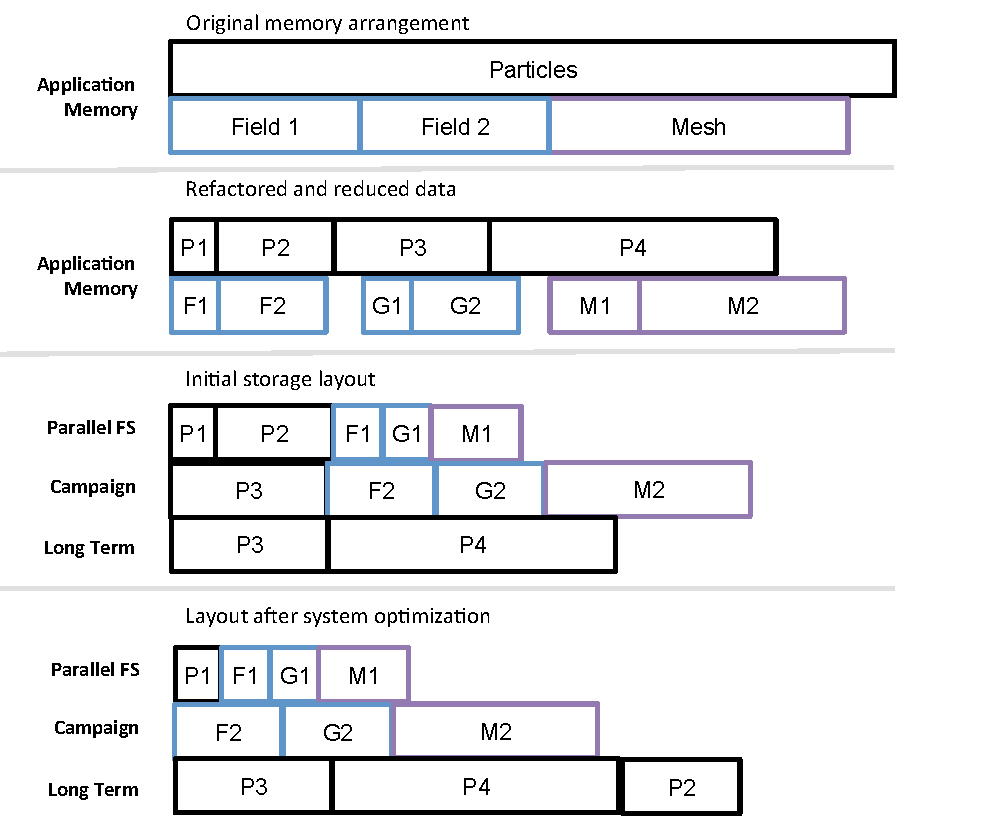
\includegraphics[scale=0.77]{graphics/SSIO-bucket.pdf}
        %\vspace{1ex}
        \caption{Data is given as a set of objects which includes utility which contains the lifetime in a storage layer, and the priority of the layer.}
        \label{fig:ssio-bucket}
        \end{centering}
%        \vspace{1ex}
\end{wrapfigure}


We will design new APIs that the users can use as part of a data mover, or the system can automatically use, to raise or lower these sub-objects
up and down the storage stack. The SSIO layer will then manage the system metadata so that the user can transparently access any of these
sub-objects without knowledge of the layer. This requires that when reading the data, the APIs will then get a time estimate of reading, and then
allow the users to determine if they will read less (only the highest priority sub-objects) if the time estimate for reading exceeds their expectations.
%

Users will also need to describe information about the data in order to choose the ``most optimal'' data-refactoring routine. Currently, we understand
that users can tell us that the data represents: 1) phase-space (e.g. the particles in our example), 2) spatial-changes (example the mesh), 3) space-time
(example the fields on the mesh). We need this information to get the best possible data refactoring methods. Although users can request 
a user-defined data-refactoring method, system-level methods can use this information to make better decisions. We will investigate new APIS 
and with new semantics to take this information and use this to best prioritize and re-organize information.

Finally we will investigate additional information on top of the data model. This information will be used to talk about data associations which go
beyond traditional data models. For example, there is a inherent relationship between the fields in our example and the mesh. A common data model
will describe all of the variables in the mesh (the coordinates, the units, the types of elements if this were a finite-element mesh) . We will explore
new mechanisms which will group data elements together so that we can understand that (M1, F1, and G1) need to be organized together. 
In otherwords, in will not be helpful if data from M1 and M2 were organized together, along with only F1. When the users wants to visualize data from 
the field, F1, they will need only M1, and M2 would be additional information. Likewise, if the user wants to see F1 and F2, then they will need the
mesh from M1 and M2, and this requires that the time to access all of this data is approximately the same, which requires that all of this needs
to be organized in the same layer of the storage system.  We will investigate what choices the SSIO system must make in order to keep these
pieces together. Do we move everything to a lower layer when all of it doesn't fit, or can we move other user-data for this data set, evict for example
P3 in order to keep F2, G2, and M2 together? We need to investigate the potential problems when this occurs, and how the users can specify
additional information to ensure they get the best possible data from the SSIO layer.


The capability of APIs provide dynamic runtime information to user and make the system 
more transparent to them rather than a black box. The end user could analyze or visualize data 
in a more comfortable position, where they are able to envision 
how much longer they are going to wait for data. 


%Firstly, we will explore the augmentation of
%I/O application programing interfaces (I/O APIs) to allow applications to
%both specify timing and quality information and also query the storage
%system for timing estimates. If user decide to write or read data to or from hierarchical storage systems, 
%they will rely on the API to send their intentions for inquiry and examine the system status, 
%including how much data they would like to write/read, desired bandwidth, data compression method, etc, 
%or the user can express their intension of writing data right now no matter what the traffic is now.
%Through this interface we expect the
%application and user to gain insights into how long a single output or input
%call will take given the required quality information, and then react to
%these estimates by adjusting the quality or restricting the scope of the
%data required. Likewise we will explore how an application can provide
%timing information to the storage system to allow the storage system to make
%optimization decisions to best meet the requirements from the application. 
%
%Secondly, we will also explore external data annotations, such as those
%provided by the configuration file in ADIOS. Through the use of these
%external augmentation the user can provide insights to the storage system on
%the relative value of the data, expected life time and performance
%characteristics, as well as relationships between different data sets. With
%this information the storage system can make optimizations specific to a use
%case. We expect these augmentations to be particularly important for
%eviction of data from a storage layer, and migration of data sets to a
%different storage layer. 



\paragraph{Challenges:}
The design of new APIs posses both technical and adoption challenges. Here
we will only consider the technical challenges. The proposed set of APIs aim
to expose broad system level environmental information to the application,
and allow the application to adapt dynamically based on this information.
One aspect of this challenge is the design of an interrogative API that
enables a back-and-forth between the application and the storage system to
enable the application to receive enough information to make adaptation
decisions.  Since we will work closely with many of the leading LCF applications we need
to make sure that our additional APIs and semantics in the SSIO layer will be accepted by them, and then
hopefully by the rest of the community. This requires that we carefully examine all possible design choices to ensure
that we don't keep changing the APIs and semantics, but we understand what we decisions can be made so that
we don't burden the users with confusing APIS and semantics which can't even be used by the system.


